
% JOD appendicies
\appendix

   %\section{Appendixes}
    \newpage
    \section{JOD Distribution}
   
   
   JOD is distributed\index{installation!distribution} as a \emph{J addon}.  
   You can install JOD using \texttt{pacman} the  
   \href{https://code.jsoftware.com/wiki/Pacman}{\emph{J package manager}} \cite{jwiki:jal}.
   
   
   The JOD distribution is broken into three \texttt{pacman} packages:
   \begin{enumerate}
	\item  \href{https://www.jsoftware.com/jwiki/Addons/general/jod}{\texttt{jod}} 
	\cite{baker:jod}:  This is the only package that must be installed to run JOD.  
	It contains  JOD system code and supporting files.
	\item  \href{https://www.jsoftware.com/jwiki/Addons/general/jodsource}{\texttt{jodsource}}
	 \cite{baker:jodsource}: This addon consists of three 
	   JOD dictionary dumps and a setup script.  JOD dictionary dumps\index{dictionary!source!\texttt{jodsource}}
	  are J script files that can rebuild  JOD dictionaries.  Dump files are the best way to
	  distribute dictionary code since they are independent of J binary representations. 
	  The \texttt{jodsource}\index{source code} addon contains.
  \begin{enumerate}
	  \item \texttt{joddev.ijs} --- development put dictionary\index{put dictionary}
	  \item \texttt{jod.ijs} --- main JOD source and test script dictionary
	  \item \texttt{utils.ijs}  --- common utilities dictionary
     \item \texttt{jodsourcesetup.ijs} --- J script that creates and loads the three
     JOD development dictionaries.
  \end{enumerate}
  \item \href{https://www.jsoftware.com/jwiki/Addons/general/joddocument}{\texttt{joddocument}} \cite{baker:joddocument}: this package contains 
  JOD PDF documents. Installing this
  package places these documents on local drives 
  for \hyperlink{il:jodhelp}{\texttt{jodhelp}}, see page~\pageref{ss:jodhelp}.  
\end{enumerate}

The \emph{packages} listed above are built from source scripts that are found in several GitHub\index{GitHub} repositories. To access raw  
JOD code see:  

\begin{enumerate}
\item The official \href{https://www.jsoftware.com}{\texttt{jsoftware.com}} repositories are:
\begin{enumerate}
\item \url{https://github.com/jsoftware/general_jod}
\item \url{https://github.com/jsoftware/general_joddocument}
\item \url{https://github.com/jsoftware/general_jodsource}
\end{enumerate}

\item My development repositories are:
\begin{enumerate}
\item \url{https://github.com/bakerjd99/jod}
\item \url{https://github.com/bakerjd99/joddumps}
\item \url{https://github.com/bakerjd99/joddoc}
\end{enumerate}

\item \LaTeX\ source for this document is at:
\begin{enumerate}
\item \url{https://github.com/bakerjd99/joddoc}
\end{enumerate}

\end{enumerate}

 \newpage
    \section{Building JOD}
    
    JOD is an open-source system. Anyone is free to examine and modify JOD source code. 
    All JOD source is stored in JOD development dictionaries. Installing the
    \href{https://www.jsoftware.com/jwiki/Addons/general/jodsource}{\texttt{jodsource}}\index{dictionary!source!\texttt{jodsource}}
    addon makes this code available. 
    
    JOD dictionaries also contain utilities for building\index{building!JOD distribution} and distributing JOD. 
    
\begin{lstlisting}[frame=single,framerule=0pt,basicstyle=\ttfamily\footnotesize]    
NB. open JOD development dictionaries
od ;:'joddev jod utils' [ 3 od ''

NB. before building create required directories
NB. directory creation is a one time step
'test' getrx 'setbuilddirs'
1 setbuilddirs_test_ 0

NB. build JOD
rm 'buildjoddistribution'
\end{lstlisting}   
    
   \texttt{buildjoddistribution} extracts JOD source code from development dictionaries and generates the compressed or 
    \href{https://en.wikipedia.org/wiki/Minification_(programming)}{\emph{minimized}} scripts 
    used by the JOD addon.
    
\begin{lstlisting}[frame=single,framerule=0pt,basicstyle=\ttfamily\footnotesize]
NB.*buildjoddistribution s-- full JOD distribution build.

cocurrent 'base'
cocurrent jodtestlocale 'AAAbuildjoddistribution'

NB. record open dictionaries and open JOD dictionaries
od ;:'joddev jod utils' [ 3 od'' [ ooo=: }. did 0

NB. get JOD build utilities and version tracking nouns
tmploc get }. grp 'buildjod'

NB. set distribution directories
jddir=: 'JODDOCDIR JODSTAGEDIR JODGITDIR JODSOURCESTAGEDIR JODSTAGEPDFDIR JODSTAGEDOCDIR'
jddir=: jddir , ' JODGITDOCDIR JODADDONDIR JODSCRIPTDIR JODEXTSDIR' 
(jddir)=: setbuilddirs 0

NB. generate distribution scripts
updatejodmanifest 0
JODVMD buildjodcompressed JODSTAGEDIR;JODGITDIR;JODADDONDIR;JODSCRIPTDIR
JODTOOLSVMD buildjodtoolscompressed JODSTAGEDIR;JODEXTSDIR;JODSCRIPTDIR
JODVMD updatejoddistribution JODSTAGEDIR;JODGITDIR;JODDOCDIR
JODVMD updatejodsourcedumps JODSOURCESTAGEDIR
JODVMD releasejod JODSTAGEDIR;JODSTAGEPDFDIR;JODSTAGEDOCDIR;JODGITDOCDIR

NB. destroy build locale
cocurrent 'base'
coerase <testlocale_ijod_
\end{lstlisting}

   \newpage
    \section{Testing JOD}\index{testing!running test scripts}

 Software is either \emph{tested} or \emph{trash}! There are no other
options! JOD aspires to be more than trash. So, it shouldn't surprise
anyone to learn that JOD development dictionaries contain many test
scripts. Test scripts are organized into \emph{suites}. Suites are
collections of test scripts.

\begin{lstlisting}[frame=single,framerule=0pt,basicstyle=\ttfamily\footnotesize]    
    NB. open JOD development dictionaries to use test scripts.
    od ;:'joddev jod utils' [ 3 od ''

    NB. make jodtester script - used by most test scripts
    mls 'jodtester'

    NB. list JOD test suites
    80 list }. 3 dnl 'jod'
jodbasictests     jodcrushtests     joddualsystests   jodextensiontests 
jodlargetests     jodmanwintests    jodpjmtest        jodpreparetests   
jodpurgetests     jodsmoketests     jodstresstests  
\end{lstlisting} 

\noindent Because test scripts are often more revealing and informative than
standard documentation, I have posted them on GitHub at

\medskip
\small \url{https://github.com/bakerjd99/jod/tree/master/jodunit}. \normalsize 
\medskip

\noindent The majority
of the scripts can be run with JOD's \hyperlink{il:rtt}{\texttt{rtt}} verb, see page~\pageref{ss:rtt}.

\begin{lstlisting}[frame=single,framerule=0pt,basicstyle=\ttfamily\footnotesize]    
    NB. run silently - only explict output shown - expected result is 1
    1 rtt 'bnlSmoke02'

    NB. show all input and output
    rtt  'bnlSmoke02'
\end{lstlisting} 

\noindent The following test script is typical of JOD tests. Run with {\texttt{rtt}}.

\begin{lstlisting}[frame=single,framerule=0pt,basicstyle=\ttfamily\footnotesize] 
NB.*bnlSmoke02 t-- (bnl) test hash failure detection.

cocurrent 'base'
require 'jodtester'

cocurrent jodtestlocale 'AAAbnlSmoke02'

testenvironment 'good';'JOD'
NB. -{TEST START}-

NB. is folder configured
iscf '~JODTEST'

NB. set test dictionary
er settdict tdict=: 'testjod00'

NB. read and write bytes
read=: 1!:1&(]`<@.(32&>@(3!:0)))
write=: 1!:2 ]`<@.(32&>@(3!:0))

NB. close any open and open test dictionary
er od tdict [ 3 od ''

NB. erase any current test dictionary backups
DL=: {: {.DPATH__ST__JODobj
0 0$ferase 1 dir BAK__DL,'*.*'

NB. no backup error expected
ner 14 bnl '.'

NB. insert random arrays  between backups to insure
NB. hashes in the njhashes.txt sidecar files differ
hashhack=: ?5 5 5$1000000
hashmsg=: 'first backup'
er tmploc put 'hashhack'
er tmploc put 'hashmsg'
er packd tdict

hashhack=: ?5 5 5$1000000
hashmsg=: 'second backup'
er tmploc put 'hashhack'
er tmploc put 'hashmsg'
er packd tdict

NB. all hashes should pass
er showpass hashes=: 17 bnl '.'
*./ ; 1 1 }. rv_ajod_ hashes

NB. copy and rename older backup word files over
NB. newer backups - this will introduce a hash failure
jwords=: dirtree BAK__DL,'*jwords.ijf'
jwords=: (\: 1 {"1 jwords){jwords
(read ;0{{:jwords) write ;0{{.jwords
er showpass hckhashes=: 17 bnl '.'

NB. some hashes fail - 0s in 17 bnl '.'
0 e. ; 1 1 }. rv_ajod_ hckhashes

NB. -{TEST SUCCESSFUL}-
ereopen 0

cocurrent 'base'
coerase <testlocale_ijod_
\end{lstlisting}   

    
     
   \newpage
   \section{JOD Classes}\label{ap:classes}
   
   \begin{figure}[htbp]
  \centering
  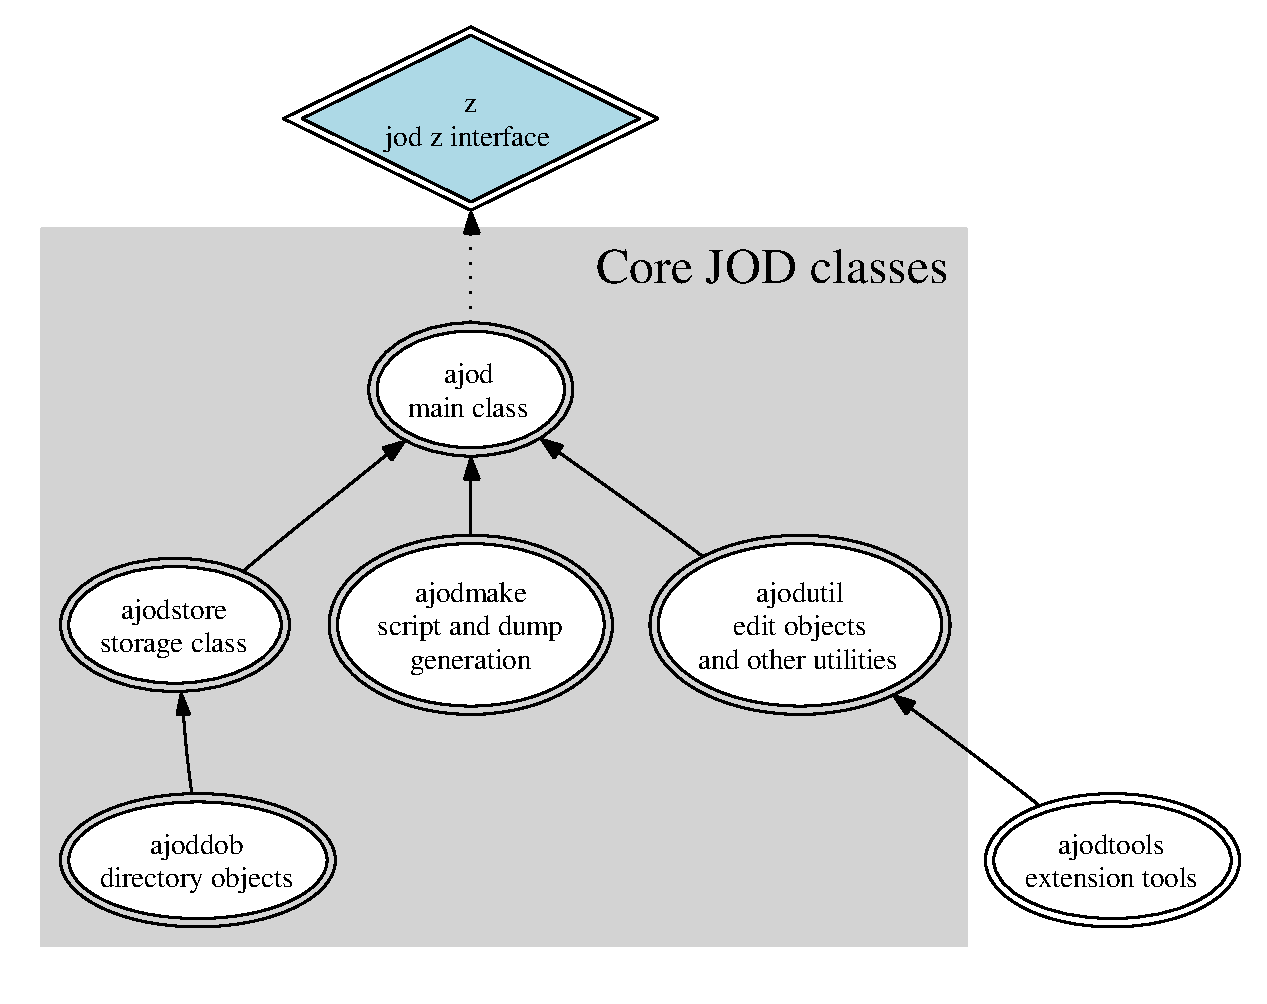
\includegraphics[width=0.84\textwidth]{joddot}
  \caption[JOD Classes]{This diagram\index{z interface}\index{ijod interface} shows how 
    JOD classes\index{classes} are related. JOD classes are loaded into 
    J addon \textbf{\texttt{a}} locales. The arrows\index{locale!classes} indicate how J names are resolved.
    The \emph{blue diamond} locales \texttt{ijod} and \texttt{z} are on the \texttt{base} locale's 
    path: \texttt{copath 'base'}. \emph{Diagram Generated by} \texttt{Graphviz} \cite{jwiki:graphviz}.    
    }
   \label{eps:joddot}
   \end{figure}
   
   \newpage
   \section{Reference Path}\label{ap:refpath}
   
   JOD groups and suites, (see \hyperlink{il:grp}{\texttt{grp}} on page~\pageref{ss:grp}), are defined with respect to a particular path.  This path is called the \emph{reference path}.  The reference path\index{reference path} is stored when the first put dictionary group or 
suite is defined.   Group and suite generation with \hyperlink{il:make}{\texttt{make}}, \hyperlink{il:mls}{\texttt{mls}} and  \hyperlink{il:lg}{\texttt{lg}}, (see pages~\pageref{ss:make}, \pageref{ss:mls}, \pageref{ss:lg}), check the current path against the reference path.  If the paths do not match an error is returned.

Reference paths display current dictionary names but the path is 
stored as a unique list of extended dictionary 
identification numbers: \texttt{DIDNUM}s.  On Windows and Linux 
systems the \texttt{DIDNUM}\index{DIDNUM} is based 
on \texttt{GUID}s.  \texttt{DIDNUM}s insure reference paths are unique.


A reference path can only be reset by clearing the put dictionary\index{put dictionary}
 path, opening desired dictionaries and recreating a group or suite: see \hyperlink{il:dpset}{\texttt{dpset}} on page~\pageref{ss:dpset}.

\begin{lstlisting}[frame=single,framerule=0pt,basicstyle=\ttfamily\footnotesize]
    NB. open first five dictionaries 
    od 5 {. }. od ''
+-+--------------------------+------+---+-----+--------+---+
|1|opened (rw/rw/ro/rw/rw) ->|budget|cbh|flick|flickdev|gps|
+-+--------------------------+------+---+-----+--------+---+

    NB. display dictionary information - reference paths in last column
    did ~ 0
+-+----------------------------------------------------------------------+
|1|+--------+--+-----+-----+-------+-------+------+---------------------+|
| ||        |--|Words|Tests|Groups*|Suites*|Macros|*Path                ||
| |+--------+--+-----+-----+-------+-------+------+---------------------+|
| ||budget  |rw|14   |0    |2      |0      |0     |/budget              ||
| |+--------+--+-----+-----+-------+-------+------+---------------------+|
| ||cbh     |rw|145  |0    |6      |0      |6     |/cbh/utils           ||
| |+--------+--+-----+-----+-------+-------+------+---------------------+|
| ||flick   |ro|296  |3    |9      |0      |9     |/flick/utils         ||
| |+--------+--+-----+-----+-------+-------+------+---------------------+|
| ||flickdev|rw|96   |2    |2      |0      |2     |/flickdev/flick/utils||
| |+--------+--+-----+-----+-------+-------+------+---------------------+|
| ||gps     |rw|11   |0    |0      |0      |0     |/gps/utils           ||
| |+--------+--+-----+-----+-------+-------+------+---------------------+|
+-+----------------------------------------------------------------------+
\end{lstlisting}
   
   \newpage
   \section{JOD Argument Codes}\label{ap:objqualcodes}

The left, and some right, arguments of JOD verbs are specified with \emph{object}, \emph{qualifier} and \emph{option} codes. Object codes\index{codes!argument} are typically the first argument code while options and qualifiers usually occupy the second and third positions. Options and qualifiers are sometimes negative. Negative values modify codes: see tables~\ref{tab:objcodes}, \ref{tab:objneg} and
\ref{tab:qualcodes} on pages~\pageref{tab:objcodes},  \pageref{tab:objneg} and \pageref{tab:qualcodes}.

\begin{table}[htbp]
  \centering
   \scriptsize
   \begin{tabular}{|l|l|l|p{4.0in}|} \hline
   \multicolumn{4}{|c|}{\textbf{\normalsize Object Codes\T\B}} \\ \hline
   \multicolumn{1}{|c|}{\textbf{\normalsize Noun\T}} & 
   \multicolumn{1}{|c|}{\textbf{\normalsize Code}} & 
   \multicolumn{1}{|c|}{\textbf{\normalsize Use}} & 
   \multicolumn{1}{|c|}{\textbf{\normalsize Example\B}} \\ \hline
   \texttt{WORD\T\B} & 0 & word code & \begin{minipage}{3.9in}
\begin{tabular}{l}
\verb|0 dnl ''  | \textcolor{CodeComment}{\ttfamily\textsl{NB. list all words on path}} \\
\end{tabular} 
\end{minipage} \\ \hline
 \texttt{TEST\T\B} & 1 & test case code & \begin{minipage}{3.9in}
\begin{tabular}{l}
\verb|1 put 'test';'test code..'  | \textcolor{CodeComment}{\ttfamily\textsl{NB. store test}} \\
\end{tabular} 
\end{minipage} \\ \hline
 \texttt{GROUP\T\B} & 2 & group code & \begin{minipage}{3.9in}
\begin{tabular}{l}
\verb|2 put 'name';'group header ...'  | \textcolor{CodeComment}{\ttfamily\textsl{NB. store group header}} \\
\end{tabular} 
\end{minipage} \\ \hline
 \texttt{SUITE\T\B} & 3 & suite code & \begin{minipage}{3.9in}
\begin{tabular}{l}
\verb|3 grp 'suite'  | \textcolor{CodeComment}{\ttfamily\textsl{NB. get suite members, list of test names}} \\
\end{tabular} 
\end{minipage} \\ \hline
 \texttt{MACRO\T\B} & 4 & macro code & \begin{minipage}{3.9in}
\begin{tabular}{l}
\verb|4 disp 'test'  | \textcolor{CodeComment}{\ttfamily\textsl{NB. display macro}} \\
\end{tabular} 
\end{minipage} \\ \hline
 \texttt{DICTIONARY\T\B} & 5 & dictionary code & \begin{minipage}{3.9in}
\begin{tabular}{l}
\verb|5 get ''  | \textcolor{CodeComment}{\ttfamily\textsl{NB. get dictionary documentation}} \\
\end{tabular} 
\end{minipage} \\ \hline
    \end{tabular}
   \caption{JOD Object Codes}
  \label{tab:objcodes}
\end{table}

The meaning of negative option and qualifier codes depends on the word.  For 
\hyperlink{il:dnl}{\texttt{dnl}} a negative option requests a \emph{path order list.}\index{path order list}
For \hyperlink{il:get}{\texttt{get}} and \hyperlink{il:put}{\texttt{put}} a negative
option code gets and puts timestamp arrays.

\begin{table}[htbp]
  \centering
   \scriptsize
\begin{tabular}{|l|l|p{4.7in}|} \hline
   \multicolumn{3}{|c|}{\textbf{\normalsize Negative Codes\T\B}} \\ \hline
   \multicolumn{1}{|c|}{\textbf{\normalsize Code\T}} & 
   \multicolumn{1}{|c|}{\textbf{\normalsize Use}} & 
   \multicolumn{1}{|c|}{\textbf{\normalsize Example\B}} \\ \hline
   \verb|_1|\T\B & path order list & \begin{minipage}{3.9in}
\begin{tabular}{l}
\verb|0 _1 dnl ''  | \textcolor{CodeComment}{\ttfamily\textsl{NB. path order list of words}} \\
\end{tabular} 
\end{minipage} \\ \hline
\verb|_2|\T\B & path order list & \begin{minipage}{3.9in}
\begin{tabular}{l}
\verb|1 _2 dnl 'boo'  | \textcolor{CodeComment}{\ttfamily\textsl{NB. path order list of test names containing boo}} \\
\end{tabular} 
\end{minipage} \\ \hline
\verb|_14|\T\B & names and timestamps & \begin{minipage}{3.9in}
\begin{tabular}{l}
\verb|1 _14 get }. revo''  | \textcolor{CodeComment}{\ttfamily\textsl{NB. names and timestamps array}} \\
\end{tabular} 
\end{minipage} \\ \hline
\verb|_14|\T\B & names and timestamps & \begin{minipage}{3.9in}
\begin{tabular}{l}
\verb|4 _14 put tsarray  | \textcolor{CodeComment}{\ttfamily\textsl{NB. update macro timestamps}} \\
\end{tabular} 
\end{minipage} \\ \hline
\end{tabular}
   \caption{JOD Negative Codes}
   \label{tab:objneg}
\end{table}

\newpage

\begin{table}[htbp]
  \centering
   \scriptsize
   \begin{tabular}{|l|l|l|p{4.0in}|} \hline
   \multicolumn{4}{|c|}{\textbf{\normalsize Qualifier Codes\T\B}} \\ \hline
   \multicolumn{1}{|c|}{\textbf{\normalsize Noun\T}} & 
   \multicolumn{1}{|c|}{\textbf{\normalsize Code}} & 
   \multicolumn{1}{|c|}{\textbf{\normalsize Use}} & 
   \multicolumn{1}{|c|}{\textbf{\normalsize Example\B}} \\ \hline
   \texttt{DEFAULT\T\B} & 7 & default action & \begin{minipage}{3.9in}
\begin{tabular}{l}
\verb|0 7 get 'this'  | \textcolor{CodeComment}{\ttfamily\textsl{NB. default behaviour}} \\
\end{tabular} 
\end{minipage} \\ \hline
 \texttt{EXPLAIN\T\B} & 8 & short explanation text & \begin{minipage}{3.9in}
\begin{tabular}{l}
\verb|0 8 put 'name';'explain name'  |  \\
\end{tabular} 
\end{minipage} \\ \hline
 \texttt{DOCUMENT\T\B} & 9 & documentation text & \begin{minipage}{3.9in}
\begin{tabular}{l}
\verb|2 9 put 'group';'very long group document ...'  |  \\
\end{tabular} 
\end{minipage} \\ \hline
 \texttt{NVTABLE\T\B} & 10 & name value table & \begin{minipage}{3.9in}
\begin{tabular}{l}
\verb|0 10 get }. dnl ''  | \textcolor{CodeComment}{\ttfamily\textsl{NB. return all words in table}} \\
\end{tabular} 
\end{minipage} \\ \hline

 \texttt{REFERENCE\T\B} & 11 & reference code & \begin{minipage}{3.9in}
\begin{tabular}{l}
\verb|11 del 'earthdist'  | \textcolor{CodeComment}{\ttfamily\textsl{NB. delete word references}} \\
\end{tabular} 
\end{minipage} \\ \hline

 \texttt{NAMECLASS\T\B} & 12 & J name class code & \begin{minipage}{3.9in}
\begin{tabular}{l}
\verb|0 12 get }. dnl ''| \textcolor{CodeComment}{\ttfamily\textsl{NB. fetch J name class codes}} \\
\end{tabular} 
\end{minipage} \\ \hline

 \texttt{CREATION\T\B} & 13 & creation date & \begin{minipage}{3.9in}
\begin{tabular}{l}
\verb|0 13 get }. dnl ''| \textcolor{CodeComment}{\ttfamily\textsl{NB. word creation dates}} \\
\end{tabular} 
\end{minipage} \\ \hline

 \texttt{LASTPUT\T\B} & 14 & last change date & \begin{minipage}{3.9in}
\begin{tabular}{l}
\verb|0 14 get }. dnl ''| \textcolor{CodeComment}{\ttfamily\textsl{NB. recent changes}} \\
\end{tabular} 
\end{minipage} \\ \hline

\texttt{HASH\T\B} & 17 & hash code & \begin{minipage}{3.9in}
\begin{tabular}{l}
\verb|17 bnl '.'| \textcolor{CodeComment}{\ttfamily\textsl{NB. check backup files against hashes}} \\
\end{tabular} 
\end{minipage} \\ \hline

 \texttt{BYTESIZE\T\B} & 15 & object byte size & \begin{minipage}{3.9in}
\begin{tabular}{l}
\verb|0 15 get }. dnl ''| \textcolor{CodeComment}{\ttfamily\textsl{NB. word byte sizes}} \\
\end{tabular} 
\end{minipage} \\ \hline

 \texttt{JSCRIPT\T\B} & 21 &  J script code\index{postprocessor} & \begin{minipage}{3.9in}
\begin{tabular}{l}
\verb|4 1 21 dnl 'POST_'  | \textcolor{CodeComment}{\ttfamily\textsl{NB. list postprocessors}} \\
\end{tabular} 
\end{minipage} \\ \hline
\texttt{LATEX\T\B} & 22 & \LaTeX\ text code  & \begin{minipage}{3.9in}
\begin{tabular}{l}
\verb|4 get }. 4 3 22 dnl 'TEX'  | \textcolor{CodeComment}{\ttfamily\textsl{NB. get LaTeX macros}} \\
\end{tabular} 
\end{minipage} \\ \hline
\texttt{HTML\T\B} & 23 & HTML text code & \begin{minipage}{3.9in}
\begin{tabular}{l}
\verb|4 put 'HTMLtxt';23;'<a>hello world</a>'  | \textcolor{CodeComment}{\ttfamily\textsl{NB. store html}} \\
\end{tabular} 
\end{minipage} \\ \hline
\texttt{XML\T\B} & 24 & XML text code & \begin{minipage}{3.9in}
\begin{tabular}{l}
\verb|4 put 'XMLtext24;'<p>baby step xml</p>'  |  \textcolor{CodeComment}{\ttfamily\textsl{NB. store xml}}\\
\end{tabular} 
\end{minipage} \\ \hline
\texttt{TEXT\T\B} & 25 & ASCII text code & \begin{minipage}{3.9in}
\begin{tabular}{l}
\verb|4 3 25 dnl 'EPS'  | \textcolor{CodeComment}{\ttfamily\textsl{NB. texts ending with EPS}} \\
\end{tabular} 
\end{minipage} \\ \hline
\texttt{BYTE\T\B} & 26 & BYTE characters & \begin{minipage}{3.9in}
\begin{tabular}{l}
\verb|4 put 'BYTEME';a.|  \\
\end{tabular} 
\end{minipage} \\ \hline

\texttt{MARKDOWN\T\B} & 27 & \href{https://daringfireball.net/projects/markdown/}{MARKDOWN} text code & \begin{minipage}{3.9in}
\begin{tabular}{l}
\verb|5 put 'Main **dictionary** document' |  \\
\end{tabular} 
\end{minipage} \\ \hline

\texttt{UTF8\T\B} & 28 & Unicode UTF8 text & \begin{minipage}{3.9in}
\begin{tabular}{l}
\verb|4 put 'UTF8text';UTF8_ajod_;(8 u: 4 u: 56788 4578,65+i.5)  |  \\
\end{tabular} 
\end{minipage} \\ \hline

\texttt{PYTHON\T\B} & 29 & Python script text & \begin{minipage}{3.9in}
\begin{tabular}{l}
\verb|4 put 'big_py';PYTHON_ajod_;'2 ** 1024'  |  \\
\end{tabular} 
\end{minipage} \\ \hline

\texttt{SQL\T\B} & 30 & SQL script text & \begin{minipage}{3.9in}
\begin{tabular}{l}
\verb|4 put 'yada_sql';SQL_ajod_;'select * from yada'  |  \\
\end{tabular} 
\end{minipage} \\ \hline

\texttt{JSON\T\B} & 31 & JSON text & \begin{minipage}{3.9in}
\begin{tabular}{l}
\verb|4 put 'fleece_json';JSON_ajod_;'{"json": "golden-fleece"}'  |  \\
\end{tabular} 
\end{minipage} \\ \hline

\texttt{IPYNB\T\B} & 32 & \href{https://jupyter.org/}{Jupyter} notebook & \begin{minipage}{3.9in}
\begin{tabular}{l}
\verb|4 put 'notebook_ipynb';IPYNB_ajod_;'... ipynb ...'  |  \\
\end{tabular} 
\end{minipage} \\ \hline

\texttt{LEAN\T\B} & 33 & \href{https://leanprover-community.github.io/}{LEAN} source code & \begin{minipage}{3.9in}
\begin{tabular}{l}
\verb|4 put 'theorem_lean';LEAN_ajod_;'... lean on me ...'  |  \\
\end{tabular} 
\end{minipage} \\ \hline

\texttt{ZIG\T\B} & 34 & \href{https://ziglang.org/}{ZIG} source code & \begin{minipage}{3.9in}
\begin{tabular}{l}
\verb|4 put 'code_zig';ZIG_ajod_;'... ziggy code stuff ...'  |  \\
\end{tabular} 
\end{minipage} \\ \hline


%\texttt{PYTHON\T\B} & 29 & Python script text & \begin{minipage}{3.9in}
%\begin{tabular}{l}
%\verb|4 put 'PYTHONTEXT';PYTHON_ajod_;'2 ** 1024'  |  \\
%\end{tabular} 
%\end{minipage} \\ \hline
    \end{tabular}
   \caption{JOD Qualifier Codes}
  \label{tab:qualcodes}
\end{table}

\textbf{Note:} suffixes like \texttt{notebook\_ipynb} are not required. I use them to make it easier to see what type of code is stored in a JOD macro.

 
   \newpage
   \section{\texttt{jodparms.ijs}}\label{ap:jodparms}
   
\verb|jodparms.ijs| is read when the master file\index{master file} \verb|jmaster.ijf| is created
and is used to set dictionary parameters.

Dictionary parameters are distributed to dictionary files and runtime
objects. New parameters can be added by editing \verb|jodparms.ijs|
and recreating the master file.
The last few lines of the following example show how to add
\texttt{COPYRIGHT} and \texttt{MYPARAMETER}. 

When a parameter is added its value will appear in the directory
objects of all dictionaries but will only be \hyperlink{il:dpset}{\texttt{dpset}}'able in new dictionaries.

\begin{quotation}
	To change default master dictionary parameters:
	\begin{enumerate}
	  \item Exit J
		\item Delete the files
	  \begin{description}
		  \item \verb|~addons/general/jod/jmaster.ijf|
		  \item \verb|~addons/general/jod/jod.ijn|
  	\end{description}
		\item Edit 
  	\begin{description}
	 	  \item \verb|~addons/general/jod/jodparms.ijs|
  	\end{description}
		\item Restart J and reload JOD with 
		\begin{description}
	   	\item \verb|load 'general/jod'|
		\end{description}
	 \end{enumerate}
\end{quotation}

%\vspace{0.5cm}	

\begin{lstlisting}[frame=single,framerule=0pt,basicstyle=\ttfamily\footnotesize]
NB.*jodparms s-- default dictionary parameters.
NB.
NB. This file is used to set  the  default  dictionary parameters
NB. table  in the master file. When  a  new dictionary is created
NB. the  parameters  in the  master file are used to specify  the
NB. parameters for a particular dictionary. The  verb (dpset) can
NB. be   used  to   modify  parameter  settings   in   individual
NB. dictionaries.  Master  file parameters can only be changed by
NB. editing this file and recreating the master file.
NB.
NB. The master file can be recreated with the call:
NB.
NB. createmast_ajod_ JMASTER_ajod_
NB.
NB. WARNING: all the  parameters currently listed are required by
NB. the JOD system. If you remove any of them JOD will crash. You
NB. can  safely add additional parameters but  you  cannot safely
NB. remove current parameters.

MASTERPARMS=: 0 : 0

NB. The format of this parameter file is:
NB.     jname ; (type) description ; value
NB. 
NB.     jname is a valid J name
NB.     (type) description documents the parameter - type is required
NB.        only (+integer) is currently executed other types will
NB.        be passed as character lists (see dptable).
NB.     value is an executable J expression that produces a value

ASCII85    ; (+integer) when 1 use ascii85 in dumps (0 or 1) ; 1  
COPYFACTOR ; (+integer) components copied in one loop pass  (1<y<240) ; 100
DOCUMENTDICT ; (+integer) when 1 dictionary document is put (0 or 1)  ; 1
DOCUMENTWIDTH ; (+integer) width of justified document text  (20<y<255) ; 61
DUMPFACTOR ; (+integer) objects dumped in one loop pass (1<y<240)     ; 50
GETFACTOR  ; (+integer) words retrieved in one loop pass (10<y<2048)  ; 250
PUTFACTOR  ; (+integer) words stored in one loop pass  (10<y<2048)    ; 100
RETAINAGE  ; (+integer) when 1 timestamps are saved in dumps (0 or 1) ; 1
HASHDUMP   ; (+integer) when 1 a hash is prefixed to dumps (0 or 1)   ; 1

NB. ROOTFOLDER is empty by default. If it is set to a (jpath) J configured 
NB. folder ROOTFOLDER overrides default locations for (mls) generated scripts 
ROOTFOLDER ; (character) redirects (mls) scripts to J folder ; 

NB. typical nonempty setting
NB. ROOTFOLDER ; (character) redirects (mls) scripts to J folder ; ~user/jodroot 

NB. Any added parameters are stored in the master file when
NB. created and distributed to JOD directory objects.  

NB. WARNING: when defining J expressions be careful about the ; character 
NB. the JOD code (dptable) that parses this string is rudimentary.

NB. COPYRIGHT ; (character) ; All rights reserved
NB. MYPARAMETER ; (+integer) the answer ; 42
)
\end{lstlisting}


   \newpage
   \section{\texttt{jodprofile.ijs}}\label{ap:jodprofile}
   
\verb|jodprofile.ijs| is an optional user profile script; it runs after
JOD loads and can be used to customize\index{configuration!\texttt{jodprofile.ijs}} your working environment.  The following is an example
profile script. 

%\lstset{numbers=left, numberstyle=\tiny, stepnumber=2, numbersep=5pt}

\begin{lstlisting}[frame=single,framerule=0pt,basicstyle=\ttfamily\footnotesize]
NB.*jodprofile s-- JOD dictionary profile.
NB.
NB. An example JOD profile script. Save this script in
NB.
NB. ~addons/general/jod/
NB.
NB. with the name jodprofile.ijs
NB.
NB. This script  is  executed  after all dictionary  objects have
NB. been created. It  can  be used  to  set up  your default  JOD
NB. working environment.

NB. set white space preservation on
9!:41 [ 1

NB. minimum print precision to show yyyymmdd dates (see jodage)
9!:11 [ 8

NB. set jqt windows console size - automatic for linux/mac/ios
Cwh_j_=: 160 24

NB. do not reset if you are running more than one JOD instance
NB. multiple JOD instances are permitted but not recommended
dpset 'RESETME'

NB. JOD interface locale - (ijod) is a good place for ad hoc JOD addons
coclass 'ijod'

NB. used by some macros: WHEREAMI=: ;0 { ;:'home work test'
WHEREAMI=: 'home'

NB. (ijod) error/ message text
ERRIJOD00=: 'current group name (jodg_ijod_) not set'
ERRIJOD01=: 'current suite name (jods_ijod_) not set'
ERRIJOD02=: 'invalid (x) search string'
OKIJOD00=:  'no matches'
OKIJOD01=:  'no objects'

NB. add delete objects from current group or current suite
ag=: {{if. wex_ajod_ <'jodg' do. jodg addgrp y else. jderr_ajod_ ERRIJOD00 end.}}
as=: {{if. wex_ajod_ <'jods' do. (jods;3) addgrp y else. jderr_ajod_ ERRIJOD01 end.}}
dg=: {{if. wex_ajod_ <'jodg' do. jodg delgrp y else. jderr_ajod_ ERRIJOD00 end.}}
ds=: {{if. wex_ajod_ <'jods' do. (jods;3) delgrp y else. jderr_ajod_ ERRIJOD01 end.}}
   
NB. referenced words not in current group
nx=: 3 : 0
if. -.wex_ajod_ <'jodg' do. jderr_ajod_ ERRIJOD00 return. end.
if. badrc_ajod_ gn=. grp jodg do. gn return. end.
(allrefs  }. gn) -. gn
)
   
NB. words in current group using a word
ug=: 3 : 0
if. -.wex_ajod_ <'jodg' do. jderr_ajod_ ERRIJOD00 return. end.
if. badrc_ajod_ gn=. grp jodg do. gn return. end.
y usedby }. gn
)
   
NB. generate current group and save load script
sg=: {{if. wex_ajod_ <'jodg' do. mls jodg else. jderr_ajod_ ERRIJOD01 end.}}

NB. open entire (y) path
oep=: 6&od

NB. top (put dictionary) words, groups, suites in revision order
tw=: revo
tg=: 2&revo
ts=: 3&revo

NB. run tautology as plaintest - does not stop on nonzero results
rt=: 2&rtt

NB. run tautology silently - will show explict smoutput
rq=:1&rtt

NB. run macro silently - will show explict smoutput
rs=: 1&rm

NB. short help for groups/suites
hg=: [: hlpnl [: }. grp
hs=: 1 hlpnl [: }. 3 grp ]

NB. short help on put objects in revised order from code:
NB.     hr 4  NB. macro
NB.     hr 2  NB. groups
NB.  10 hr 0  NB. last ten words
hr=: 3 : 0
if. badrc_ajod_ w=. y revo '' do. w return. end.
y hlpnl }. w
:
if. badrc_ajod_ w=. y revo '' do. w return. end.
y hlpnl x {. }. w
)

NB. remove trailing blank rows
rebtbrow=: ] #~ [: -. [: *./"1 [: *./\. ' '&=

NB. appends trailing line feed character if necessary
tlf=:] , ((10{a.)"_ = {:) }. (10{a.)"_

NB. show long documents
NB.      hld 0     NB. words
NB.      hld 2     NB. groups
NB.  0 1 0 hld 0   NB. documented nouns
NB. 'NIMP:' hld 0  NB. word docs with string 'NIMP:'
NB.  (] ,: #@hld"0) i. 5 NB. count docs on path
hld=: ''&$: :(4 : 0)
if. badcl_ajod_ x do. jderr_ajod_ ERRIJOD02 return. end.
if. badrc_ajod_ w=. y dnl '' do. w return. end.
if. 0=#&> w=. }. w do. ok_ajod_ OKIJOD01 return. end.
if. badrc_ajod_ d=. (({.y),9) get w do. d return. end.
d=. d #~ 0 < #&> 1 {"1 d=. >1{d
if. 0<#x do. d=. d #~ +./@(x&E.)&> 1 {"1 d end.
(0 {"1 d) ,. rebtbrow@(];._2)@tlf@(-.&CR)&.> 1 {"1 d
)

NB. search short help for string and list matching words
NB.     hss 'see long'   NB. search word short text 
NB.  2  hss 'see long'   NB. search group short text
NB.  4  hss 'post'       NB. search macro short text 
hss=: 0&$: :(4 : 0)
if. badrc_ajod_ w=. x dnl ''   do. w return. end.
d=. x hlpnl }. w
if. 0=#w=. 1 >@{ d             do. ok_ajod_ OKIJOD00 return. end.
if. 0=#s=. I. (,:y) +./"1@E. w do. ok_ajod_ OKIJOD00 return. end.
s&{ &.> d
)

NB. single line explanation 
NB.    slex 'word'         NB. word
NB.  4 slex 'jodregister'  NB. macro
NB.  1 slex 'thistest'     NB. test
slex=: 0&$: :(4 : 0)
if. badcl_ajod_ sl=. x disp y do. sl return. end.
(x,8) put y;firstcomment__JODtools sl
)

NB. regenerate put dictionary word cross references
reref=: 3 : 0
if. badrc_ajod_ r=. revo '' do. r return. end.
(r,.s) #~ -.;0{"1 s=.0 globs&> r=.}.r
)

NB. handy cl doc helpers
docscr=: {{ctl_ajod_ (61;0;0;'NB.') docct2__UT__JODobj ];._1 LF,y-.CR}}
doctxt=: {{ctl_ajod_ (61;0;0;'') docct2__UT__JODobj ];._1 LF,y-.CR}}

NB. display noun on screen and return noun value
showpass=:] [ 1!:2&2

NB. portable box drawing characters
portchars=:[: 9!:7 '+++++++++|-'"_ [ ]

NB. windows lucida console box drawing characters
winlcchars=:[: 9!:7 (a.{~16+i.11)"_ [ ]

NB. edit command 
DOCUMENTCOMMAND=: 'showpass pr ''{~N~}'''

NB. read & write files
read=:1!:1&(]`<@.(32&>@(3!:0)))
write=:1!:2 ]`<@.(32&>@(3!:0))
readnoun=:3!:2@(1!:1&(]`<@.(32&>@(3!:0))))
writenoun=:([: 3!:1 [) (1!:2 ]`<@.(32&>@(3!:0))) ]

NB. fetch edit text/macros and associate code
tt=:] ; gt
mt=:] ; 25"_ ; gt   NB. *.txt
mj=:] ; 21"_ ; gt   NB. *.ijs
md=:] ; 27"_ ; gt   NB. *.markdown
mq=:] ; 30"_ ; gt   NB. *.sql
mx=:] ; 22"_ ; gt   NB. *.tex

NB. ~user/temp object text - default j script
os=: 'ijs'&$: : ([: jpath '~user/temp/' , (' ' -.~ ]) , '.' , ' ' -.~ [)
 
NB. read text from j user temp directory
jt=:[: read os
 
NB.  load j script from j user temp
jl=: (0!:0)@jt

NB. load j script from configured j path
jp=: [: 0!:0 [: < jpath

NB. load and show j script from configured path
jps=: [: 0!:001 [: < jpath

NB. number of objects - used by various (utils) macros (sizeput, ageput, ...) if present
NOBS=: 10

NB. show (1) or suppress (0) dyadic (smoutput)
SHOWSMO=: 1

NB. create temporary named and labeled jod test locales for j 9.6 and beyond
NB. NOTE: WARNING: (jodtestlocale) is used in most JOD test scripts.
(3 : 0) ''
if. 9.6 <: jvn_ajod_'' do.
jodtestlocale=: {{'ijod' jodtestlocale y 
: 
((;:x),copath y) copath y [ _1 cocreate <y [ coerase <y=. y -. ' '
('tmploc_',y,'_')=: y [ testlocale_ijod_=:y}}
else.
jodtestlocale=: {{'ijod' jodtestlocale y 
: 
((;:x),copath y) copath y [ cocreate <y [ coerase <y=. y -. ' '
('tmploc_',y,'_')=: y [ testlocale_ijod_=: y}}
end.
'jodtestlocale defined'
)

NB. clear vestigal JOD objects during load - this value must exist
NB. and match 1 for vestigal objects to be cleared by (createjod)
CLEARVOBS=: 1

NB. clear dictionaries - used by (utils) macro (clearput) if present
NB. CLEARJDICS=: ;:''

NB. set a preferred local pandoc  - used by (jodliterate) - try (where pandoc)
NB. PREFERREDPANDOC=: 'C:\Users\genric.user\AppData\Local\Pandoc\pandoc'
NB. PREFERREDPANDOC=: '/usr/local/bin/pandoc'

NB. JOD verbs typically run from the base locale 
cocurrent 'base'
\end{lstlisting}

   \newpage
   \section{\texttt{joduserconfigbak.ijs}}\label{ap:jodusercfgbak}
   
\verb|joduserconfigbak.ijs| is an optional configuration\index{configuration!\texttt{joduserconfigbak.ijs}} 
script. \verb|joduserconfigbak.ijs| is in the directory.
\begin{verbatim}
  ~addons/general/jod/jodbak
\end{verbatim}
\verb|joduserconfigbak.ijs| can be used to redefine class words before
any JOD objects are created. 
   
\begin{lstlisting}[frame=single,framerule=0pt,basicstyle=\ttfamily\footnotesize]  
NB.*joduserconfigbak s-- example JOD user configuration script.
NB.
NB. This  script is  executed BEFORE JOD objects  are created. It
NB. can be used to redefine and customize various class words. To
NB. make  this script  active  rename it to (joduserconfig.ijs) and
NB. copy it, with your edits, to the main jod directory:
NB.
NB. ~addons/general/jod
NB.
NB. The nouns listed below are good candidates for redefinition.

smoutput 'joduserconfig.ijs executing ...'

NB. PDF reader in jodutil class - Reset for other PDF readers
PDFREADER_ajodutil_=:'C:\Adobe\Acrobat Reader DC\Reader\AcroRd32.exe'

NB. Reset J's PDF reader to match JOD's PDF reader - do for (jconsole.exe)
PDFReader_j_=: PDFREADER_ajodutil_

NB. Alternative Ghostscript compatible reader
NB. PDFREADER_ajodutil_=:'C:\Program Files\Ghostgum\gsview\gsview32.exe'

NB. Preferred web browser in jodutil class - default Windows FireFox directory
WWW0_ajodutil_=:'C:\Program Files\Mozilla Firefox\firefox.exe'

NB. Secondary web browser in jodutil class - default Windows directory
WWW1_ajodutil_=:'C:\Program Files\Internet Explorer\IEXPLORE.EXE'

NB. Text editor to use when running JOD in (jconsole.exe) on Windows systems
NB. QT/JHS configurations are not necessarily applied for (jconsole,exe)
EDCONSOLE_ajodutil_=:'"C:\Program Files (x86)\notepad++\notepad++.exe"'
\end{lstlisting}

   
   \newpage
   \section{JOD \texttt{startup.ijs} entries}\label{ap:startup}
   
\verb|startup.ijs| is J's optional user startup\index{configuration!\texttt{startup.ijs}} 
script. \verb|startup.ijs| is in the directory.
\begin{verbatim}
  ~config   
\end{verbatim}
JOD uses \verb|startup.ijs|
to store load scripts generated by \hyperlink{il:mls}{\texttt{mls}}: see page~\pageref{ss:mls}.
   
\begin{lstlisting}[frame=single,framerule=0pt,basicstyle=\ttfamily\footnotesize]   
NB. WARNING: JOD managed section do not edit!
NB.<JOD_Load_Scripts>
buildpublic_j_ 0 : 0
bstats  c:/jod/jutils/script/bstats.ijs
xmlutils  c:/jod/utils/script/xmlutils.ijs
analystgraphs  c:/jod/franklin/script/analystgraphs.ijs
TeXfrWpxml  c:/jod/docs/script/TeXfrWpxml.ijs
jodtester  c:/jod/joddev/script/jodtester.ijs
waypoints  c:/jod/gps/script/waypoints.ijs
Weeks  c:/jod/docs/script/Weeks.ijs
MirrorXref  c:/jod/smugpyter/script/MirrorXref.ijs
DudTeXPreprocess  c:/jod/docs/script/DudTeXPreprocess.ijs
BiblioHelper  c:/jod/docs/script/BiblioHelper.ijs
RecodeSchedZ  c:/jod/mwecc/script/RecodeSchedZ.ijs
)
NB.</JOD_Load_Scripts>
\end{lstlisting}

\newpage
\section{Turning JOD Dump Script Tricks}\label{ap:joddumptricks}

Dump script generation is my favorite JOD feature. Dump scripts serialize 
JOD dictionaries; they are mainly used to backup dictionaries and interact with 
version control systems: see appendix~\ref{ap:jodvcsys} on page~\pageref{ap:jodvcsys}.
However, dump scripts are general J scripts and can do much more!  
Maintaining a stable of healthy JOD dictionaries is easier 
if you can turn a few dump script tricks.\footnote{Spicing up one's rhetoric with a double entendre 
like ``turning tricks'' may be construed as a 
\href{http://thefederalist.com/2015/03/24/microaggressions-and-trigger-warnings-meet-real-trauma/}{\emph{microaggression}}. 
The point of colored language is to memorably make a point. 
You are unlikely to forget \emph{turning dump script tricks.} 
}

\begin{enumerate}

\item \textbf{Flattening reference paths:} Open JOD dictionaries define a reference path: see appendix~\ref{ap:refpath} on page~\pageref{ap:refpath}.
For example, if you open the following dictionaries:

\begin{lstlisting}[frame=single,framerule=0pt,basicstyle=\ttfamily\footnotesize]
   NB. open four dictionaries
   od ;:'smugdev smug image utils'
+-+-----------------------+-------+----+-----+-----+
|1|opened (ro/ro/ro/ro) ->|smugdev|smug|image|utils|
+-+-----------------------+-------+----+-----+-----+
\end{lstlisting}

The reference path is \texttt{/smugdev/smug/image/utils}.

When objects are retrieved each dictionary on the path is searched in reference path order.
If there are \emph{no compelling reasons} to maintain separate dictionaries you can improve
JOD retrieval performance and simplify dictionary maintenance by flattening all or part of the path. 

To flatten the reference path do:

\begin{lstlisting}[frame=single,framerule=0pt,basicstyle=\ttfamily\footnotesize]
   NB. reopen first three dictionaries on path
   od ;:'smugdev smug image' [ 3 od ''
+-+--------------------+-------+----+-----+
|1|opened (ro/ro/ro) ->|smugdev|smug|image|
+-+--------------------+-------+----+-----+

   NB. dump to a temporary file (df)
   df=: {: showpass make jpath '~temp/smugflat.ijs'
+-+---------------------------+--------------------------------------------+
|1|object(s) on path dumped ->|c:/users/john/j64-803-user/temp/smugflat.ijs|
+-+---------------------------+--------------------------------------------+

   NB. create a new flat dictionary
   newd 'smugflat' [ 3 od ''
+-+---------------------+--------+---------------------------------------------+
|1|dictionary created ->|smugflat|c:/users/john/j64-803-user/joddicts/smugflat/|
+-+---------------------+--------+---------------------------------------------+

   NB. open the flat dictionary and (utils)
   od ;:'smugflat utils'
+-+-----------------+--------+-----+
|1|opened (rw/ro) ->|smugflat|utils|
+-+-----------------+--------+-----+
  
   NB. load the dump script 
   0!:0 df
\end{lstlisting}

The collapsed path \texttt{/smugflat/utils} will return the same objects as the longer path.
It is important to understand that the collapsed dictionary \texttt{smugflat} does not necessarily contain
the same objects found in the three original dictionaries \texttt{smugdev}, \texttt{smug} and \texttt{image}.
If objects with the same name exist in the original dictionaries only the first one found will 
be in the collapsed dictionary.


\item \textbf{Merging dictionaries:} If two dictionaries \emph{contain no overlapping objects} it might make
sense to merge them. This is easily achieved with dump scripts. To merge two or more dictionaries do:

\begin{lstlisting}[frame=single,framerule=0pt,basicstyle=\ttfamily\footnotesize]
   NB. open and dump first dictionary
   od 'dict0' [ 3 od ''
+-+--------------+-----+
|1|opened (rw) ->|dict0|
+-+--------------+-----+
   df0=: {: showpass make jpath '~temp/dict0.ijs'
+-+---------------------------+-----------------------------------------+
|1|object(s) on path dumped ->|c:/users/john/j64-803-user/temp/dict0.ijs|
+-+---------------------------+-----------------------------------------+
   
   NB. open and dump second dictionary
   od 'dict1' [ 3 od ''
+-+--------------+-----+
|1|opened (rw) ->|dict1|
+-+--------------+-----+
   df1=: {: showpass make jpath '~temp/dict1.ijs'
+-+---------------------------+-----------------------------------------+
|1|object(s) on path dumped ->|c:/users/john/j64-803-user/temp/dict1.ijs|
+-+---------------------------+-----------------------------------------+
   
   NB. create new merge dictionary
   newd 'mergedict' [ 3 od ''
+-+---------------------+---------+----------------------------------------------+
|1|dictionary created ->|mergedict|c:/users/john/j64-803-user/joddicts/mergedict/|
+-+---------------------+---------+----------------------------------------------+
   
   NB. open merge dictionary and run dump scripts
   od 'mergedict'
+-+--------------+---------+
|1|opened (rw) ->|mergedict|
+-+--------------+---------+
   0!:0 df0  NB. .... output omitted ... 
   0!:0 df1
\end{lstlisting}

Be careful when merging dictionaries. If there are common objects the last object loaded is the one
retained in the merged dictionary.



\item \textbf{Updating master dictionary parameters:} When a new dictionary parameter is added to \texttt{jodparms.ijs}, 
see () on page () it will not be available in existing dictionaries.
\end{enumerate} 



\newpage


\section{JOD Direct Definition Support}\label{ap:jodddef}

J version 9.02 (February 2021) introduced \index{direct definition} \emph{direct definitions}. The
designers of APL languages, of which J is a member, introduced direct definitions
long after \emph{canonical} or notorious ``$\pmb\triangledown$ editor'' style definitions. In retrospect,
most agree the entire family of languages would be better off if direct definition
had come first. Direct definitions are more elegant, concise, versatile, and beautiful than
clunky canonical equivalents. They're also easier to comprehend and compose than
long J tacit definitions. But history is history, and software history is hard to ignore because of the \emph{installed base}\footnote{Also known as \emph{users}}.
We're stuck with our kludges!

In JOD's case this shows up in how \hyperlink{il:globs}{\texttt{globs}}, see page~\pageref{ss:globs}, classifies global and local names in words
that contain direct definitions.  Consider the following:


\begin{lstlisting}[frame=single,framerule=0pt,basicstyle=\ttfamily\footnotesize]
make_my_def=: 3 : 0

NB. local to make_my_def
here=. we=. 2 + are=. 3 * local=. 4

global_adv=: {{*./"1 u/&> 2 <\"1 y}}

local_verb=. {{)d
  NB. not local to make_my_def
  we=. are=. not=. make_my_def=. local=. x
  if. 1-:y do.
    NB. deep global to make_my_def
    {{deep_gbl=: 'deep';":y}} y  
  end.
}}

0 local_verb y
)
\end{lstlisting}

\texttt{make\_my\_def} contains local and global direct definitions. When executed it creates  \texttt{global\_adv}
and runs \texttt{local\_verb} which in turn creates \texttt{deep\_gbl}.  When \texttt{local\_verb} runs it creates
a local namespace like any explicit J verb. Hence \texttt{not} and \texttt{make\_my\_def}  are not \emph{strictly} \texttt{make\_my\_def} locals.  \emph{The
execution of  directly defined local words is equivalent to calling explicit words.}  \texttt{globs} does not track direct definition name scopes. 
It views all direct definition names as if they belonged to the topmost word.  For \texttt{make\_my\_def}  \texttt{globs} this gives:

\begin{lstlisting}[frame=single,framerule=0pt,basicstyle=\ttfamily\footnotesize]   
   NB. JOD name classification
   11 globs 'make_my_def' 
\end{lstlisting}

\newpage

\begin{lstlisting}[frame=single,framerule=0pt,basicstyle=\ttfamily\footnotesize]   
+-+-------------------------------------------------------+
|1|+------+----------------------------------------------+|
| ||Global|+--------+----------+                         ||
| ||      ||deep_gbl|global_adv|                         ||
| ||      |+--------+----------+                         ||
| |+------+----------------------------------------------+|
| ||Local |+---+----+-----+----------+-----------+---+--+||
| ||      ||are|here|local|local_verb|make_my_def|not|we|||
| ||      |+---+----+-----+----------+-----------+---+--+||
| |+------+----------------------------------------------+|
| ||(*)=: |                                              ||
| |+------+----------------------------------------------+|
| ||(*)=. |                                              ||
| |+------+----------------------------------------------+|
| ||for.  |                                              ||
| |+------+----------------------------------------------+|
+-+-------------------------------------------------------+
   
   NB. execute and show name classes
   make_my_def 1
+----+-+
|deep|1|
+----+-+
   nc ;:'local_verb global_adv deep_gbl' 
_1 1 0
\end{lstlisting}

When embedding direct defintions in explicit words, or within other direct definitions, it's a good idea to make names distinct.
For example, in embedded \texttt{local\_verb} do something like:

\begin{lstlisting}[frame=single,framerule=0pt,basicstyle=\ttfamily\footnotesize]   
local_verb=. {{)d
  weLv=. areLv=. notLv=. make_my_defLv=. localLv=. x
  if. 1-:y do.
    NB. deep global to make_my_def
    {{deep_gbl=: 'deep';":y}} y  
  end.
}}
\end{lstlisting}











\newpage
\section{JOD and Version Control Systems}\label{ap:jodvcsys}

Despite JOD's backup and restore facilities, see \texttt{bnl}, \texttt{bget}, \texttt{packd} and
\texttt{restd} on pages \pageref{ss:bnl}, \pageref{ss:bget}, \pageref{ss:packd} and \pageref{ss:restd}, JOD is not 
a  source code version control system like \href{http://git-scm.com/}{\texttt{Git}}\index{version control!\texttt{Git}} \cite{gitsite} or 
\href{http://subversion.tigris.org/}{\texttt{Subversion}}\index{version control!\texttt{Subversion}} \cite{subvsite}. 
 JOD's primary
purpose is efficiently  refactoring, shuffling and recombining J words not tracking their detailed histories. 
\emph{Traditional version control systems focus on the history
of source code} and provide detailed  merge, security and multiuser network 
facilities that JOD  lacks.  However, since JOD generates
standard J source code scripts it's easy to use JOD with version control systems. 
The main difficulty is choosing a suitable level of detail: \emph{dictionary, script} or \emph{word.} 
The following shows how \texttt{Git} can be used for each of these levels. \texttt{Git} has
a number of graphical \texttt{GUI} interfaces these examples use 
\href{http://www.gnu.org/software/bash/manual/bashref.html}{bash shell} commands.

\begin{enumerate}
\item \textbf{Dictionary:}\label{it:dictlev} \texttt{make}, see page~\pageref{ss:make}, can dump entire
dictionaries as a single J script. Dump scripts contain all\footnote{Word references 
are not present in dump scripts. They can
be easily regenerated with \texttt{globs}, see page~\pageref{ss:globs}.} dictionary word definitions,
test scripts, groups, suites and macros. Storing dump scripts in version control systems is
an effective and simple way of tracking dictionary changes.  To create dump scripts I run
the macro \texttt{dumpput}.
\texttt{dumpput} is stored in the \texttt{utils} dictionary; it dumps the put dictionary and
copies the generated script to a common local directory. The common local directory
hosts a \texttt{Git} repository that has a \href{https://github.com/bakerjd99/joddumps}{\texttt{GitHub}} remote repository set.
A remote \texttt{GitHub}  repository is good way to move dictionaries between machines
and safely share them with others. In the following example local changes
are committed and then pushed to a remote repository.\footnote{A collection of JOD dictionary dump scripts is available at: \href{https://github.com/bakerjd99/joddumps}{\texttt{https://github.com/bakerjd99/joddumps}.}
}


\begin{lstlisting}[frame=single,framerule=0pt,basicstyle=\ttfamily\footnotesize]
   NB. Step 1: J session commands - open dictionaries
   od ;:'docs utils' [ 3 od ''
+-+-----------------+----+-----+
|1|opened (rw/ro) ->|docs|utils|
+-+-----------------+----+-----+
   
   1 rm 'dumpput'  NB. run dump macro - (utils) must be on path
+-+---------------------------+-------------------------+
|1|object(s) on path dumped ->|c:/jod/docs/dump/docs.ijs|
+-+---------------------------+-------------------------+
+------------------------+
|c:/jod/joddumps/docs.ijs|
+------------------------+
\end{lstlisting}

\begin{lstlisting}[language=bash,frame=single,framerule=0pt
,basicstyle=\ttfamily\footnotesize,backgroundcolor=\color{CodeBackGround}]
$ echo Step 2: Bash shell commands > /dev/null

bakerjd99@NINJA /c/jod/joddumps (master)
$ pwd
/c/jod/joddumps

bakerjd99@NINJA /c/jod/joddumps (master)
$ git status -s
M  docs.ijs
 M joddev.ijs
 M utils.ijs

bakerjd99@NINJA /c/jod/joddumps (master)
$ git commit -m 'recent changes to docs.ijs dictionary'
[master 1577d1a] recent changes to docs.ijs dictionary
 1 files changed, 46 insertions(+), 4 deletions(-)
 
bakerjd99@NINJA /c/jod/joddumps (master) 
$ git remote
joddumps
origin

bakerjd99@NINJA /c/jod/joddumps (master) 
$ git push joddumps master 
\end{lstlisting}

\item \textbf{Script:} Word and test scripts generated by JOD are stored
in a dictionary's  \texttt{script} and \texttt{suite} subdirectories, see Figure~\ref{eps:joddirs} on page~\pageref{eps:joddirs}.
In the following a \texttt{Git} repository has been created in the \texttt{script} subdirectory
and the contents of the \texttt{exim} group have been edited and regenerated.

\begin{lstlisting}[frame=single,framerule=0pt,basicstyle=\ttfamily\footnotesize]
   NB. Step 1: J session commands - open dictionaries
   od ;:'smugdev smug image utils' [ 3 od ''
+-+-----------------------+-------+----+-----+-----+
|1|opened (rw/ro/ro/ro) ->|smugdev|smug|image|utils|
+-+-----------------------+-------+----+-----+-----+

   NB. edit (exim) content and save changes ...
   
   NB. regenerate (exim) script
   mls 'exim'
+-+--------------------+------------------------------+
|1|load script saved ->|c:/jod/smugdev/script/exim.ijs|
+-+--------------------+------------------------------+
\end{lstlisting}

\begin{lstlisting}[language=bash,frame=single,framerule=0pt
,basicstyle=\ttfamily\footnotesize,backgroundcolor=\color{CodeBackGround}]
$ echo Step 2: Bash shell commands > /dev/null

bakerjd99@NINJA /c/jod/smugdev/script (master)
$ pwd
/c/jod/smugdev/script

bakerjd99@NINJA /c/jod/smugdev/script (master)
$ git status -s
 M exim.ijs

bakerjd99@NINJA /c/jod/smugdev/script (master)
$ git add exim.ijs

bakerjd99@NINJA /c/jod/smugdev/script (master)
$ git commit -m '(masspixels) added to description of (exim) interface'
[master e93ffe5] (masspixels) added to description of (exim) interface
 1 files changed, 13 insertions(+), 11 deletions(-)
\end{lstlisting}

\item \textbf{Word:} JOD does not directly generate individual word scripts 
but it is easy to define
a simple utility that does. \texttt{pwf}\footnote{
\texttt{pwf} is not a complete solution to exporting 
individual JOD objects as scripts. It only exports words
 and ignores tests, groups, macros and other objects.
It does not address the issue of synchronizing exported
objects with dictionary state. For example, dictionary word
deletions are not propagated. If you wish to track 
dictionary state use the \textbf{\texttt{Dictionary}} (\pageref{it:dictlev})
level method.}
writes individual JOD put dictionary
word files. \texttt{pwf} is stored in the \texttt{utils} dictionary.

\begin{lstlisting}[frame=single,framerule=0pt,basicstyle=\ttfamily\footnotesize]
pwf=:3 : 0

NB.*pwf v-- write path dictionary words as script files.
NB.
NB. monad:  pwf clPattern
NB.
NB.   pwf ''    NB. write all path dictionary words
NB.
NB. dyad:   clPath pwf clPattern
NB.
NB.   'c:/temp' pwf 'de' NB. write to given directory

'' pwf y
:
NB. JOD references !(*)=. dnl get badrc_ajod_ ok_ajod_ 
NB. !(*)=. isempty_ajod_ jpathsep_ajod_ makedir_ajod_ write_ajod_
pk=.  >@{                        
tsl=. ] , ('\'"_ = {:) }. '\'"_  
if. badrc_ajod_ ws=. 0 _1 dnl y        do. ws return. end.
if. badrc_ajod_ ws=. 0 10 get 1 pk ws  do. ws return. end.
NB. individual word scripts using short description text for tacits
if. badrc_ajod_ ws=. 0 0 1 wttext__MK__JODobj 1 pk ws  do. ws return. end.
try.
  NB. if (x) path is empty use put dictionary directory (alien\words)
  if. isempty_ajod_ x do.
    DL=. {:{.DPATH__ST__JODobj NB. !(*)=. DL
    NB. insure subdirectory when (x) is empty
    NB. when (x) is nonempty assume it exists
    makedir_ajod_ <jpathsep_ajod_ tsl x=. ALI__DL,'words'
  end.
  NB. write individual word files
  ws=. 1 pk ws
  wpf=. (<jpathsep_ajod_ tsl x) ,&.> (0 {"1 ws) ,&.> <'.ijs'
  ok_ajod_ wpf [ (toHOST&.> 1 {"1 ws) write_ajod_&.> wpf
catchd. jderr_ajod_ 'unable to write all word file(s)'
end.
)
\end{lstlisting}

Using \texttt{pwf} is a simple matter of getting and running it.  The following
exports  \texttt{joddev} words  to \verb|joddev/alien/words| 
and then commits differences in \texttt{Git}.

\begin{lstlisting}[frame=single,framerule=0pt,basicstyle=\ttfamily\footnotesize]
   NB. Step 1: J session commands - open dictionaries
   od ;:'joddev jod utils' [ 3 od ''
+-+--------------------+------+---+-----+
|1|opened (rw/ro/ro) ->|joddev|jod|utils|
+-+--------------------+------+---+-----+

   NB. load (pwf, showpass) into the (ijod) locale
   'ijod' get ;:'pwf showpass'
+-+-----------------+
|1|2 word(s) defined|
+-+-----------------+

   NB. edit/modify/create words and save changes ...

   #showpass pwf ''  NB. write and count word files
+-+-------------------------------------+...
|1|c:/jod/joddev/alien/words/ASCII85.ijs|...
+-+-------------------------------------+...
121
\end{lstlisting}

\begin{lstlisting}[language=bash,frame=single,framerule=0pt
,basicstyle=\ttfamily\footnotesize,backgroundcolor=\color{CodeBackGround}]
$ echo Step 2: Bash shell commands > /dev/null

bakerjd99@NINJA /c/jod/joddev/alien/words (master)
$ pwd
/c/jod/joddev/alien/words

bakerjd99@NINJA /c/jod/joddev/alien/words (master)
$ git status -s
 M pwf.ijs

bakerjd99@NINJA /c/jod/joddev/alien/words (master)
$ git add pwf.ijs

bakerjd99@NINJA /c/jod/smugdev/script (master)
$ git commit -m '(pwf) comments added'
[master e93fga4] (pwf) comments added
 1 files changed, 3 insertions(+), 2 deletions(-)
\end{lstlisting}







\end{enumerate}  
  
\newpage
\section{Hungarian Notation for J}\label{ap:jodhung}
   
\begin{figure}[htbp]
  \centering
  \href{http://www.zippythepinhead.com/}{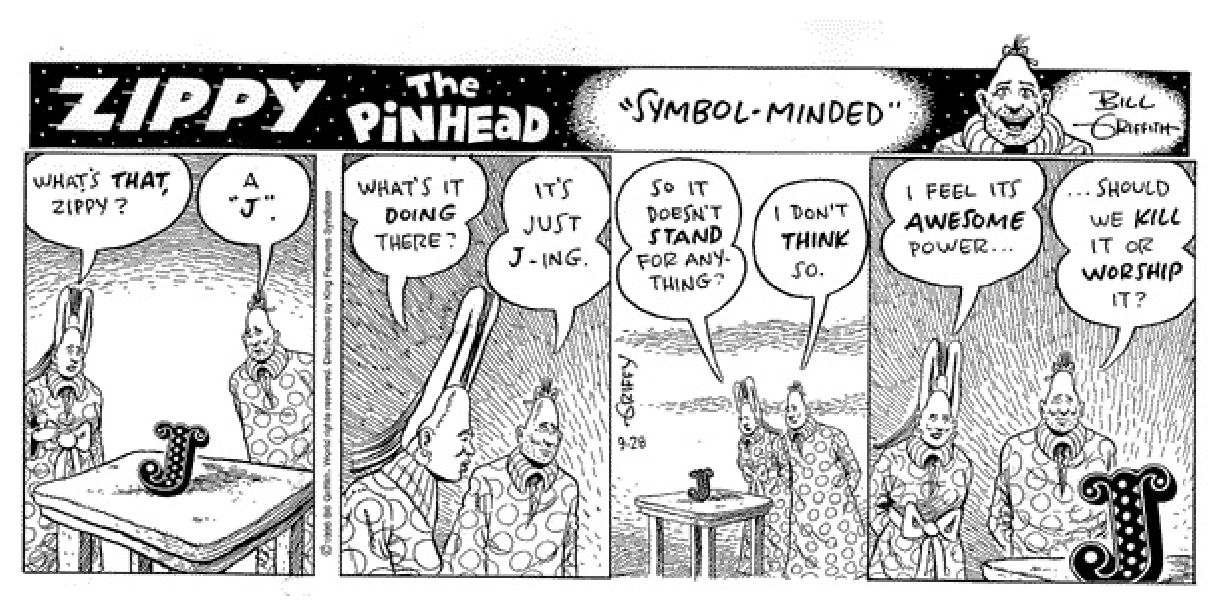
\includegraphics[width=0.8\textwidth]{zippy}}
  \caption[Zippy the Pinhead]{Zippy\index{Zippy} \cite{zippy} isn't the only one challenged by the \emph{awesome power} of J.}
  \label{eps:zippy}
\end{figure}

\subsection{Whither Hungarian}

J is a \emph{dynamically typed} language!  What this means is that
you do not have to declare the types of arguments and that types
can change during program execution.  Discarding the 
type declaration machinery found in other programming languages simplifies
J coding but it can impose its own problems. Without declarations
it's not always clear \emph{what is a valid argument}.  J does
not require that you provide hints and, in J's \emph{tacit} case, it
does not even require that you provide arguments!  Given
the language's terse nature this quickly leads to an incomprehensible
style that J detractors have dubbed \emph{line noise}. 

To distinguish my J code from line noise I have adapted a documentation
style known as \href{http://en.wikipedia.org/wiki/Hungarian_notation}{Hungarian notation} \cite{wiki:hung}. 
 Hungarian notation inspires devotion and disgust.  Many swear by it and many
 swear at it.  For me a
convention is worthwhile if it \emph{helps me} understand code.  The style
outlined here helps me understand and maintain J code.  It might help you too.

\subsection{J Noun Types}

There are two broad classes of arguments in J: nouns and verbs.  Nouns are data;
they correspond to arguments found in other programming languages.  Verbs are programs.  J adverbs
and conjunctions take verb arguments.\footnote{Adverbs and conjunctions also take noun
arguments.} Adverbs and conjunctions roughly correspond to the
higher order functions found in languages like
\href{http://www.cs.cmu.edu/Groups/AI/html/cltl/cltl2.html}{\texttt{LISP}} \cite{commonlisp} and
\href{http://www-swiss.ai.mit.edu/projects/scheme/}{\texttt{Scheme}} \cite{scheme}. 
J \emph{explicit} definition syntax reserves the characters \texttt{x y m n
u v} for arguments: see Table~\ref{tab:jargs} on page~\pageref{tab:jargs}.\footnote{
Earlier versions of J used  \texttt{ x.\ y.\ m.\ n.\ u.\ v.\ } for arguments.  This inflected
syntax has been deprecated.} The Hungarian notation described here focuses on noun arguments, 
(\texttt{x} and \texttt{y}), because they are the most common.

\begin{table}[htbp]
  \centering
   \scriptsize
\begin{tabular}{|l|l|} \hline
   \multicolumn{2}{|c|}{\textbf{\normalsize J Explicit Arguments\T\B}} \\ \hline
   \texttt{x\T\B} & \textcolor{CodeComment}{\ttfamily\textsl{left verb noun argument}}  \\
   \texttt{y\T\B} & \textcolor{CodeComment}{\ttfamily\textsl{right verb noun argument}} \\ 
   \texttt{m\T\B} & \textcolor{CodeComment}{\ttfamily\textsl{left conjunction noun argument}} \\ 
   \texttt{n\T\B} & \textcolor{CodeComment}{\ttfamily\textsl{right conjunction noun argument}} \\ 
   \texttt{u\T\B} & \textcolor{CodeComment}{\ttfamily\textsl{left adverb/conjunction verb argument}} \\ 
   \texttt{v\T\B} & \textcolor{CodeComment}{\ttfamily\textsl{right conjunction verb argument}}  \\ \hline
\end{tabular}
   \caption[J Arguments]{Characters reserved for J \emph{explicit} definition arguments. \emph{Tacit} definitions do
   not directly refer to arguments.}
   \label{tab:jargs}
\end{table}

To succinctly describe a J noun you need to be mindful of:
\begin{itemize}
	\item Type
	\item Rank
	\item Boxing
\end{itemize}

\textbf{J types} are congruent to simple types in other languages.  The standard J utility verb \texttt{datatype} enumerates primitive J noun types.

\begin{lstlisting}[frame=single,framerule=0pt,basicstyle=\ttfamily\footnotesize] 
datatype=: 3 : 0
  n=. 1 2 4 8 16 32 64 128 1024 2048 4096 8192 16384 32768 65536 131072 262144
  t=. '/boolean/literal/integer/floating/complex/boxed/extended/rational'
  t=. t,'/sparse boolean/sparse literal/sparse integer/sparse floating'
  t=. t,'/sparse complex/sparse boxed/symbol/unicode/unicode4'
  (n i. 3!:0 y) pick <;._1 t
)

  NB. types of list items
  datatype&.> (2x^128);1;'char';(s: ' symbol minded');7 %~ i. 4 5
+--------+-------+-------+------+--------+
|extended|boolean|literal|symbol|floating|
+--------+-------+-------+------+--------+
\end{lstlisting}  

\textbf{Rank} has a precise technical meaning in J but in this context it can be loosely
thought of as array dimension.   Typical ranks in J are:
\begin{itemize}
	\item Single numbers like \texttt{42} and characters \texttt{'a'} are called atoms. They
	have \textsl{rank 0}.\footnote{\textsl{Rank 0}, or \textsl{0-dimensional} objects occur in
	in all programming languages but are \emph{rarely recognized.} This leads to mountains of ugly special case code. J is more than a programming language; it's a comprehensive and rigorous way 
to \emph{think} about arrays.} 
	\item Lists like \verb|1 2 3| and \verb|'characters'| correspond to \textsl{1-dimensional} arrays
	in most languages and have \textsl{rank 1}.
	\item Tables like \verb|i. 3 2| are \textsl{2-dimensional} arrays and have \textsl{rank 2}.  
	\item $n$ dimensional arrays have rank $n$.
\end{itemize}

\textbf{Boxing} is structural.  J nouns are either boxed or simple.  A  simple noun
has one of the types, (excluding boxed), listed by
the \texttt{datatype} verb.  To mix types in a J array you must box.
\begin{lstlisting}[frame=single,framerule=0pt] 
      NB. you must box < to mix types in J arrays
      (<u: 'unicode me'),(<i. 2 3),<'types to mix'
\end{lstlisting}  

\subsection{Hungarian Noun Descriptions}

To describe J nouns I use the following rules:\footnote{As in
the film \emph{Pirates of the Caribbean} these rules are more like \emph{guidelines!}} 

\begin{figure}
  \centering
  \ttfamily
  \scriptsize
  \subfigure[J native type prefixes]{
\begin{tabular}{|l|l|l|} \hline
   \multicolumn{3}{|c|}{\rmfamily\textbf{\normalsize J Native Type Prefixes\T\B}} \\ \hline
   \multicolumn{1}{|c|}{\rmfamily\textbf{Prefix\T\B}} &
   \multicolumn{1}{|c|}{\rmfamily\textbf{Native Type\T\B}} &
   \multicolumn{1}{|c|}{\rmfamily\textbf{ \texttt{(3!:0)} code\T\B}} \\ \hline
 p\T\B & \textcolor{CodeComment}{\textsl{boolean}}   &      1  \\    
 c\T\B & \textcolor{CodeComment}{\textsl{literal}}   &      2  \\    
 i\T\B & \textcolor{CodeComment}{\textsl{integer}}   &      4  \\    
 f\T\B & \textcolor{CodeComment}{\textsl{floating}}  &      8  \\    
 j\T\B & \textcolor{CodeComment}{\textsl{complex}}   &      16 \\    
 b\T\B & \textcolor{CodeComment}{\textsl{boxed}}    &      32 \\    
 X\T\B & \textcolor{CodeComment}{\textsl{extended}}  &      64 \\    
 R\T\B & \textcolor{CodeComment}{\textsl{rational}}  &      128  \\  
 SP\T\B & \textcolor{CodeComment}{\textsl{sparse boolean}} & 1024  \\ 
 SC\T\B & \textcolor{CodeComment}{\textsl{sparse literal}} &  2048 \\  
 SI\T\B & \textcolor{CodeComment}{\textsl{sparse integer}} &  4096  \\ 
 SF\T\B & \textcolor{CodeComment}{\textsl{sparse floating}} & 8192 \\  
 SJ\T\B & \textcolor{CodeComment}{\textsl{sparse complex}}  & 16384 \\ 
 SB\T\B & \textcolor{CodeComment}{\textsl{sparse boxed}}    & 32768 \\ 
 s\T\B  & \textcolor{CodeComment}{\textsl{symbol}}          & 65536  \\                 
 w\T\B  & \textcolor{CodeComment}{\textsl{unicode}}         & 131072 \\ 
 W\T\B  & \textcolor{CodeComment}{\textsl{unicode4}}        & 262144 \\ \hline
\end{tabular}
  }
  \hspace{0.6cm} %\hfill
  \subfigure[Generic prefixes]{
  \begin{tabular}{|l|l|} \hline
   \multicolumn{2}{|c|}{\rmfamily\textbf{\normalsize Generic Prefixes\T\B}} \\ \hline
   \multicolumn{1}{|c|}{\rmfamily\textbf{Prefix\T\B}} &
   \multicolumn{1}{|c|}{\rmfamily\textbf{Description \T\B}} \\ \hline
 n\T\B & \textcolor{CodeComment}{\textsl{any numeric type including boolean}}  \\   
 N\T\B & \textcolor{CodeComment}{\textsl{any extended numeric type}}  \\
 u\T\B & \textcolor{CodeComment}{\textsl{universal - any J type}}  \\    
 z\T\B & \textcolor{CodeComment}{\textsl{empty - has at least one 0 axis}}  \\ \hline 
\end{tabular}
  }
  \caption[Hungarian Type Prefixes]{\rmfamily Hungarian type prefixes.}
  \label{fig:hungtype}
\end{figure}

\begin{enumerate}
	\item For basic descriptions I use \textsl{TypeRank[Name]}  where \textsl{Type} comes
	from Figure~\ref{fig:hungtype} on page~\pageref{fig:hungtype}, \textsl{Rank} is one of: 
	\begin{center}
	 \footnotesize
\begin{tabular}{ll}
   \texttt{a} & \textcolor{CodeComment}{\ttfamily\textsl{atom - rank 0}} \\ 
   \texttt{l} & \textcolor{CodeComment}{\ttfamily\textsl{list - rank 1}}  \\
   \texttt{t} & \textcolor{CodeComment}{\ttfamily\textsl{table - rank 2}} \\   
   \texttt{[n]} & \textcolor{CodeComment}{\ttfamily\textsl{general rank $n$}} \\ 
\end{tabular}
\end{center}
and \textsl{Name} is an optional descriptive name.  The \textsl{TypeRank} prefix uses
the case of Figure~\ref{fig:hungtype} on page~\pageref{fig:hungtype} and \textsl{Name} begins with an uppercase letter.
 \begin{center}
 \footnotesize
\begin{tabular}{ll}
   \texttt{paSwitch} & \textcolor{CodeComment}{\ttfamily\textsl{boolean (proposition) Switch}} \\ 
   \texttt{ilColors} & \textcolor{CodeComment}{\ttfamily\textsl{integer list Colors}}  \\
   \texttt{ctDocument} & \textcolor{CodeComment}{\ttfamily\textsl{character table Document}} \\   
   \texttt{jt} & \textcolor{CodeComment}{\ttfamily\textsl{complex numerix table or matrix}} \\ 
   \texttt{s[3]Xref} & \textcolor{CodeComment}{\ttfamily\textsl{rank 3 array of Xref symbols}} \\ 
   \texttt{Rl} & \textcolor{CodeComment}{\ttfamily\textsl{extended rational list}} \\ 
   \texttt{bt} & \textcolor{CodeComment}{\ttfamily\textsl{boxed table}} \\
   \texttt{SClRare} & \textcolor{CodeComment}{\ttfamily\textsl{sparse character list Rare}} \\
   \texttt{wlPersian} & \textcolor{CodeComment}{\ttfamily\textsl{unicode list Persian}} \\ 
   \texttt{ztHolder} & \textcolor{CodeComment}{\ttfamily\textsl{empty table Holder}} \\ 
   \texttt{ulWhatever} & \textcolor{CodeComment}{\ttfamily\textsl{universal list - any J list}} \\ 
   \texttt{uu} & \textcolor{CodeComment}{\ttfamily\textsl{universal universal - any J argument}} \\ 
\end{tabular}
\end{center}
 \item For boxed nouns of depth one I use a \textsl{TypeRankTypeRank[Name]} where the right most      pairing describes the boxed types.  Boxed nouns of depth one occur often.
 \begin{center}
 \footnotesize
\begin{tabular}{ll}
   \texttt{blcl} & \textcolor{CodeComment}{\ttfamily\textsl{boxed list of character lists}} \\ 
   \texttt{blit} & \textcolor{CodeComment}{\ttfamily\textsl{boxed list of integer tables}}  \\
   \texttt{bljtCoord} & \textcolor{CodeComment}{\ttfamily\textsl{boxed list of complex tables}} \\   
   \texttt{blul} & \textcolor{CodeComment}{\ttfamily\textsl{boxed list any lists}} \\ 
   \texttt{b[3]s[4]Maps} & \textcolor{CodeComment}{\ttfamily\textsl{boxed rank 3 array of rank 4 symbol array Maps }} \\ 
\end{tabular}
\end{center} 
 \item For more complex nouns, when it's helpful to expose some external structure, I use
 a mixture of more basic noun descriptions and J syntax. 
  \begin{center}
 \footnotesize
\begin{tabular}{ll}
   \texttt{(<blcl),<jtPlane} & \textcolor{CodeComment}{\ttfamily\textsl{two item list}} \\ 
   \texttt{pa;ftXy;<btuu} & \textcolor{CodeComment}{\ttfamily\textsl{three item list}}  \\
   \texttt{cl;ia;(<blcl),<blcl} & 
     \textcolor{CodeComment}{\ttfamily\textsl{see Table~\ref{tab:juses} page~\pageref{tab:juses}}} \\
   \texttt{itYYYYMMDD;slWords;(<bt),<clName} &
     \textcolor{CodeComment}{\ttfamily\textsl{four item list}} \\
   \texttt{saRed,saGreen,saBlue} & 
     \textcolor{CodeComment}{\ttfamily\textsl{emphasize items of simple noun}} \\
\end{tabular} 
\end{center}
 \item Finally, when more than one description is needed I separate individual 
 descriptions with the \emph{or} symbol \argsep and use as many consecutive lines as required.\footnote{The \argsep symbol was chosen because it falls outside 
 of J's ASCII vocabulary and suggests ``either-or.''} 
  \begin{center}
 \footnotesize
\begin{tabular}{l}
 \textcolor{CodeComment}{\ttfamily\textsl{dyadic \hyperlink{il:put}{put} argument description see page~\pageref{ss:put}}} \\
 \texttt{iaObject put clName \argsep blclNames \argsep btNvalues} \\
 \texttt{clLocale put clName \argsep blclNames \argsep btNvalues} \\
 \texttt{(iaObject,iaQualifier) put clName \argsep blclNames}  \\
 \texttt{(iaObject,iaQualifier) put clName \argsep btNvalues} \\
 \\
  \textcolor{CodeComment}{\ttfamily\textsl{dyadic \hyperlink{il:dnl}{dnl} argument description see page~\pageref{ss:dnl}}} \\
 \texttt{iaObject dnl zl \argsep clPstr} \\
 \texttt{(iaObject,iaOption) dnl zl \argsep clPstr} \\
  \texttt{(iaObject,iaOption,iaQualifier) dnl zl } \\
  \texttt{(iaObject,iaOption,iaQualifier) dnl clPstr} \\
\end{tabular} 
\end{center}
\end{enumerate}

\newpage
\section{JOD Mnemonics}

%\centering
\large
\itshape
  
\href{https://www.acronymfinder.com/Mnemonics-Neatly-Eliminate-Man's-Only-Nemesis-_-Insufficient-Cerebral-Storage-(MNEMONICS).html}{``\textbf{M}nemonics \textbf{N}eatly \textbf{E}liminate \textbf{M}an's \textbf{O}nly \textbf{N}emesis - \textbf{I}nsufficient \textbf{C}erebral \textbf{S}torage.''}

\Large

\begin{center}

	\hyperlink{il:jodhelp}{jodhelp} us!
	
	I \hyperlink{il:get}{get} it!

   \hyperlink{il:dnl}{dnl} is not just a river in Egypt.
   
   And Jesse \hyperlink{il:bget}{bget} old code.
	
	\hyperlink{il:put}{put} it where the sun don't shine.
	
	\hyperlink{il:make}{make} my day.

   \hyperlink{il:globs}{globs} of gunk.
	
	We're living in a golden \hyperlink{il:jodage}{jodage}.
	
	\hyperlink{il:did}{did}dle me this!
	
	\hyperlink{il:grp}{grp}'ing in the dark.
	
	Am I going to live \hyperlink{il:doc}{doc}?
	
	It was \hyperlink{il:revo}{revo}lting.
	
	He \hyperlink{il:od}{od}'ed man.
	
	\hyperlink{il:et}{et} phone home.
	
	It's a brand \hyperlink{il:newd}{newd}.
	
	He put on a fine \hyperlink{il:disp}{disp}lay.
	
	Dick \hyperlink{il:uses}{uses} Jane.
	
	I feel well \hyperlink{il:restd}{restd}.
	
	All \hyperlink{il:packd}{packd} up and nowhere to go.
	
	\hyperlink{il:bget}{bget} me a backup \href{https://www.youtube.com/watch?v=69iB-xy0u4A}{shrubbery}.
\end{center}

\normalsize	
\normalfont	

%\newpage
%\section{Web \texttt{URLS}}
%% urls embedded in document source.  This contents of this file
% has been derived from the output of J word (extracthrefs}
     
\begin{description}
                
\item  \emph{The JOD Pages}.\index{URL}  This website maintains references to all
JOD related documents and downloads.

\jodurl{http://bakerjd99.googlepages.com/home}
                                 
\item Wikipedia entry for \emph{Hungarian Notation}:  it's tedious and overwrought
but conveys the essentials.

\jodurl{http://en.wikipedia.org/wiki/Hungarian_notation}
                       
\item The website of the legendary computer scientist Donald Knuth.  Knuth created
the typesetting language \TeX\ in the
1970's and \TeX\ is still in widespread use because nothing
developed since is any better.  Genius is hard to replace!

\jodurl{http://www-cs-faculty.stanford.edu/~knuth/}
                            
\item All about the \emph{Scheme} programming language. 

 \jodurl{http://www-swiss.ai.mit.edu/projects/scheme/}
                          
\item \emph{Common Lisp} is the industrial strength version of the \texttt{LISP}
family of programming languages.  It's star has been waning since
the late 1980's.  

\jodurl{http://www.cs.cmu.edu/Groups/AI/html/cltl/cltl2.html}
                  
\item The  website for \emph{Graphviz}.  Graphviz is an amazing open source
system that draws graphs.  Some of the diagrams in this document were
generated with Graphviz using the J Graphviz addon.

\jodurl{http://www.graphviz.org}
                                               
\item J documentation for the \texttt{scriptdoc} utility.  

\jodurl{http://www.jsoftware.com/help/user/scriptdoc.htm}
                      
\item J Wiki download page for the \texttt{jodsource} addon.\index{Addon}

\jodurl{http://www.jsoftware.com/jwiki/Addons/general/jodsource}
               
\item J Wiki download page for the \texttt{jod} addon.

\jodurl{http://www.jsoftware.com/jwiki/Addons/general/jod}

\item J Wiki download page for the \texttt{graphviz} addon. After JOD this is
my favorite J addon. Oleg Kobchenko has created a jewel for J users!

\jodurl{http://www.jsoftware.com/jwiki/Addons/graphics/graphviz}

\item Oleg's J Page.  Chock full of interesting examples of J programming.

\jodurl{http://olegykj.sourceforge.net/}
                     
\item J Wiki addon list.  This is a complete list of J addons.

\jodurl{http://www.jsoftware.com/jwiki/Addons}
                                 
\item J Wiki documentation about JAL: the J package manager.  JAL is
the main tool for downloading and installing J addons. 

\jodurl{http://www.jsoftware.com/jwiki/JAL/Package_Manager}
                                              
\item Main J page.  This is were you go to download the latest version of J.  

\jodurl{http://www.jsoftware.com}
                                              
\item A hard copy spiral bound book version of this document is available 
here.  The price of the book is at cost. 

\jodurl{http://www.lulu.com/content/3229961}

\end{description}


%\input{jodsource}

	
